\documentclass[11pt]{article}
\usepackage{comment} %includecomment{Antwort} oder excludecomment{Antwort}
\usepackage[ngerman]{babel}\usepackage[babel=true]{microtype}
\usepackage[utf8]{inputenc}
\usepackage[T1]{fontenc}
\usepackage{lmodern}
\usepackage[a4paper,includeheadfoot,
	top=2cm, 
	bottom=2cm, 
	left=2cm, 
	right=2cm]{geometry}
\usepackage{color}
\usepackage{listings}
\usepackage[tikz]{mdframed}%\begin{mybox} \end{mybox}
\usepackage{amsmath,amssymb,amsfonts,amsthm}
\usepackage{graphicx} %\includegraphics[width=0.7\textwidth]{bild.jpg}
\usepackage{placeins} %for \FloatBarrier
\usepackage{caption} 
\usepackage[colorlinks=false,pdfborder={0 0 0}]{hyperref}%Hide RED PDF Border
\usepackage[showonlyrefs]{mathtools}%Math equations erstellen: \numberthis \label{key} abrufen:\ref{key}\eqref{key}
\usepackage{sectsty}
\usepackage{fancyhdr}\pagestyle{fancy}
\usepackage{xcolor} \definecolor{hintergrund}{HTML}{B0C4E3} \definecolor{cobalt}{rgb}{0.0, 0.28, 0.67}


\DeclareMathOperator*{\argmin}{argmin}
\DeclareMathOperator*{\argmax}{argmax}

\newcommand\numberthis{\addtocounter{equation}{1}\tag{\theequation}}
%%%%%%%%%%%%%%%%%%%%%%%%%%%%%%%%%%%%%%%%%%%%%%%%%%%%%%%%%%%%%%%%%%%
%                 Erstellt von Matthias Duch 2017                 %
%                                                                 %
% Programmiersprachen: (ausser den Standardsprachen)              %
% LaTeX, R, Stata                                                 %
%    \%%%%%%%%%%%%%%%%%%%%%%%%%%%%%%%%%%%%%%%%%%%%%%%%%%%%%%%%%%%%%%%%%%%
%                 Erstellt von Matthias Duch 2017                 %
%                                                                 %
% Programmiersprachen: (ausser den Standardsprachen)              %
% LaTeX, R, Stata                                                 %
%    \\input{../1.Vorlesung/Folien/settingsListing}               %
%%%%%%%%%%%%%%%%%%%%%%%%%%%%%%%%%%%%%%%%%%%%%%%%%%%%%%%%%%%%%%%%%%%
\usepackage{listings}
\definecolor{yellow}{RGB}{181,137,0}
\definecolor{red}{RGB}{220,50,47}
\definecolor{violet}{RGB}{108,113,196}
\definecolor{green}{rgb}{0,0.6,0}
\definecolor{gray}{rgb}{0.5,0.5,0.5}

\definecolor{Rblue}{HTML}{0000FF}
\definecolor{myblue}{HTML}{0000FF}




\newcommand{\colcomment}{\color{green}}
\newcommand{\colkeyword}{\color{blue}}
\newcommand{\coltexelem}{\color{green}}
\newcommand{\colnumbers}{\color{gray}}
\newcommand{\colstrings}{\color{violet}}
\newcommand{\colbackgrd}{\color{white}}

\lstset{literate= % Sonderzeichen ersetzen
  {á}{{\'a}}1 {é}{{\'e}}1 {í}{{\'i}}1 {ó}{{\'o}}1 {ú}{{\'u}}1
  {Á}{{\'A}}1 {É}{{\'E}}1 {Í}{{\'I}}1 {Ó}{{\'O}}1 {Ú}{{\'U}}1
  {à}{{\`a}}1 {è}{{\`e}}1 {ì}{{\`i}}1 {ò}{{\`o}}1 {ù}{{\`u}}1
  {À}{{\`A}}1 {È}{{\'E}}1 {Ì}{{\`I}}1 {Ò}{{\`O}}1 {Ù}{{\`U}}1
  {ä}{{\"a}}1 {ë}{{\"e}}1 {ï}{{\"i}}1 {ö}{{\"o}}1 {ü}{{\"u}}1
  {Ä}{{\"A}}1 {Ë}{{\"E}}1 {Ï}{{\"I}}1 {Ö}{{\"O}}1 {Ü}{{\"U}}1
  {â}{{\^a}}1 {ê}{{\^e}}1 {î}{{\^i}}1 {ô}{{\^o}}1 {û}{{\^u}}1
  {Â}{{\^A}}1 {Ê}{{\^E}}1 {Î}{{\^I}}1 {Ô}{{\^O}}1 {Û}{{\^U}}1
  {œ}{{\oe}}1 {Œ}{{\OE}}1 {æ}{{\ae}}1 {Æ}{{\AE}}1 {ß}{{\ss}}1
  {ű}{{\H{u}}}1 {Ű}{{\H{U}}}1 {ő}{{\H{o}}}1 {Ő}{{\H{O}}}1
  {ç}{{\c c}}1 {Ç}{{\c C}}1 {ø}{{\o}}1 {å}{{\r a}}1 {Å}{{\r A}}1
  {€}{{\euro}}1 {£}{{\pounds}}1 {«}{{\guillemotleft}}1
  {»}{{\guillemotright}}1 {ñ}{{\~n}}1 {Ñ}{{\~N}}1 {¿}{{?`}}1
}

\usepackage{accsupp}    
\lstset {
    numberstyle=\tiny\noncopynumber,
}

\newcommand{\noncopynumber}[1]{
    \BeginAccSupp{method=escape,ActualText={}}
    #1
    \EndAccSupp{}
}

% globale Einstellungen
\lstset{ %
  backgroundcolor=\colbackgrd,   % choose the background color; 
  basicstyle=\footnotesize,        % the size of the fonts that are used for the code
  breakatwhitespace=false,         % sets if automatic breaks should only happen at whitespace
  breaklines=true,                 % sets automatic line breaking
  emptylines=1, 
  captionpos=b,                    % sets the caption-position to bottom
  commentstyle=\itshape\colcomment,    % comment style
  deletekeywords={...},            % if you want to delete keywords from the given language
 % escapeinside={\%*}{*)},          % if you want to add LaTeX within your code
  extendedchars=true,              % lets you use non-ASCII characters; for 8-bits encodings only, does not work with UTF-8
  frame=single,	                   % adds a frame around the code
  keepspaces=true,                 % keeps spaces in text, useful for keeping indentation of code (possibly needs columns=flexible)
  keywordstyle=\colkeyword,       % keyword style
  otherkeywords={*,...},           % if you want to add more keywords to the set
  numbers=left,                    % where to put the line-numbers; possible values are (none, left, right)
  numbersep=1pt,                   % how far the line-numbers are from the code
  numberstyle=\sffamily\tiny\color{red!90}\noncopynumber, % the style that is used for the line-numbers
  numberfirstline=true,
  rulecolor=\color{black!70},         % if not set, the frame-color may be changed on line-breaks within not-black text (e.g. comments (green here))
  showspaces=false,                % show spaces everywhere adding particular underscores; it overrides 'showstringspaces'
  showstringspaces=false,          % underline spaces within strings only
  showtabs=false,                  % show tabs within strings adding particular underscores  showtabs=false,                 , % show tabs within strings adding particular underscores
  stepnumber=1,                    % the step between two line-numbers. If it's 1, each line will be numbered
  stringstyle=\colstrings,     % string literal style
  tabsize=2,	                   % sets default tabsize to 2 spaces
  title=\lstname,                   % show the filename of files included with \lstinputlisting; also try caption instead of title
  xleftmargin=3.4pt, % Einschub, durch die Zeilennummerierung bedingt
  xrightmargin=3.4pt,
  %
  alsoletter={.},
  %
  basicstyle=\ttfamily\color{black}, 
  columns=flexible,
}

%%%%%%%%%%%%%%%%%%%%%%%%%%%%%%%%%%%%%%%%%%%%%%%%%%%%%%%%%%%%%%%%%%%
%                           Sprachdefinitionen                    %
%%%%%%%%%%%%%%%%%%%%%%%%%%%%%%%%%%%%%%%%%%%%%%%%%%%%%%%%%%%%%%%%%%%

\lstdefinelanguage{Stata}{
    morekeywords=,
    morekeywords=[2]{cntrade, chinafin, wbopendata, spmap,},
    morekeywords=[3]{regress, summarize, display,},
    morekeywords=[4]{forvalues, if, foreach, set},
    morekeywords=[5]{rnormal, runiform},
    morecomment=[l]{//},
    morecomment=[s]{/*}{*/},
    % The following is used by macros, like `lags'.
    morecomment=[n][keywordstyle]{`}{'},
    morestring=[b]",
    sensitive=true,
}

\lstdefinestyle{Stata}{
  language=Stata,
  keywordstyle=\color{black},
  moredelim=**[is][\color{red}]{@}{@},
}

\lstdefinestyle{R}{%eigentlich nur R, aber aus Kompatibilitat zu alten Versionen
  style=base
}
\newcommand{\CodeSymbol}[1]{\textcolor{red}{#1}}

\lstdefinestyle{base}{
  language=R,
  emptylines=1,
  breaklines=true,
  alsoletter={.},
  basicstyle=\ttfamily\color{black},
  keywordstyle=\color{black},
  moredelim=**[is][\color{red}]{@}{@},
  %otherkeywords={<-,!,!=,~,$,*,\&,+,^,\%,\%/\%,\%*\%,\%\%,<<-,_,/},
%  morekeywords=,
%  morekeywords=[2]{+, chinafin, wbopendata, spmap,},
}

\lstdefinestyle{Latex}{
  language={[LaTeX]TeX},
  %
  moretexcs={geometry, definecolor, textcolor, colorbox, color, pagecolor, fcolorbox, setlength, tableofcontents, subsection, subsubsection, thepage, includegraphics, listoftables, citet, citep, eqref, fnysmbol, nameref, listoffigures, listoftables, url, href, printindex, blindtext, pause, titlepage, frametitle, subtitle, titlepage, usetheme,}, % define Commands
  morekeywords={maketitle}, %Keywords
  %
  texcsstyle=*\coltexelem, % Commandstyle
  moredelim=**[s][\color{yellow}]{[}{]},
}

%Patch issue, that closing parenthesis is not colored, if breaklines=True


               %
%%%%%%%%%%%%%%%%%%%%%%%%%%%%%%%%%%%%%%%%%%%%%%%%%%%%%%%%%%%%%%%%%%%
\usepackage{listings}
\definecolor{yellow}{RGB}{181,137,0}
\definecolor{red}{RGB}{220,50,47}
\definecolor{violet}{RGB}{108,113,196}
\definecolor{green}{rgb}{0,0.6,0}
\definecolor{gray}{rgb}{0.5,0.5,0.5}

\definecolor{Rblue}{HTML}{0000FF}
\definecolor{myblue}{HTML}{0000FF}




\newcommand{\colcomment}{\color{green}}
\newcommand{\colkeyword}{\color{blue}}
\newcommand{\coltexelem}{\color{green}}
\newcommand{\colnumbers}{\color{gray}}
\newcommand{\colstrings}{\color{violet}}
\newcommand{\colbackgrd}{\color{white}}

\lstset{literate= % Sonderzeichen ersetzen
  {á}{{\'a}}1 {é}{{\'e}}1 {í}{{\'i}}1 {ó}{{\'o}}1 {ú}{{\'u}}1
  {Á}{{\'A}}1 {É}{{\'E}}1 {Í}{{\'I}}1 {Ó}{{\'O}}1 {Ú}{{\'U}}1
  {à}{{\`a}}1 {è}{{\`e}}1 {ì}{{\`i}}1 {ò}{{\`o}}1 {ù}{{\`u}}1
  {À}{{\`A}}1 {È}{{\'E}}1 {Ì}{{\`I}}1 {Ò}{{\`O}}1 {Ù}{{\`U}}1
  {ä}{{\"a}}1 {ë}{{\"e}}1 {ï}{{\"i}}1 {ö}{{\"o}}1 {ü}{{\"u}}1
  {Ä}{{\"A}}1 {Ë}{{\"E}}1 {Ï}{{\"I}}1 {Ö}{{\"O}}1 {Ü}{{\"U}}1
  {â}{{\^a}}1 {ê}{{\^e}}1 {î}{{\^i}}1 {ô}{{\^o}}1 {û}{{\^u}}1
  {Â}{{\^A}}1 {Ê}{{\^E}}1 {Î}{{\^I}}1 {Ô}{{\^O}}1 {Û}{{\^U}}1
  {œ}{{\oe}}1 {Œ}{{\OE}}1 {æ}{{\ae}}1 {Æ}{{\AE}}1 {ß}{{\ss}}1
  {ű}{{\H{u}}}1 {Ű}{{\H{U}}}1 {ő}{{\H{o}}}1 {Ő}{{\H{O}}}1
  {ç}{{\c c}}1 {Ç}{{\c C}}1 {ø}{{\o}}1 {å}{{\r a}}1 {Å}{{\r A}}1
  {€}{{\euro}}1 {£}{{\pounds}}1 {«}{{\guillemotleft}}1
  {»}{{\guillemotright}}1 {ñ}{{\~n}}1 {Ñ}{{\~N}}1 {¿}{{?`}}1
}

\usepackage{accsupp}    
\lstset {
    numberstyle=\tiny\noncopynumber,
}

\newcommand{\noncopynumber}[1]{
    \BeginAccSupp{method=escape,ActualText={}}
    #1
    \EndAccSupp{}
}

% globale Einstellungen
\lstset{ %
  backgroundcolor=\colbackgrd,   % choose the background color; 
  basicstyle=\footnotesize,        % the size of the fonts that are used for the code
  breakatwhitespace=false,         % sets if automatic breaks should only happen at whitespace
  breaklines=true,                 % sets automatic line breaking
  emptylines=1, 
  captionpos=b,                    % sets the caption-position to bottom
  commentstyle=\itshape\colcomment,    % comment style
  deletekeywords={...},            % if you want to delete keywords from the given language
 % escapeinside={\%*}{*)},          % if you want to add LaTeX within your code
  extendedchars=true,              % lets you use non-ASCII characters; for 8-bits encodings only, does not work with UTF-8
  frame=single,	                   % adds a frame around the code
  keepspaces=true,                 % keeps spaces in text, useful for keeping indentation of code (possibly needs columns=flexible)
  keywordstyle=\colkeyword,       % keyword style
  otherkeywords={*,...},           % if you want to add more keywords to the set
  numbers=left,                    % where to put the line-numbers; possible values are (none, left, right)
  numbersep=1pt,                   % how far the line-numbers are from the code
  numberstyle=\sffamily\tiny\color{red!90}\noncopynumber, % the style that is used for the line-numbers
  numberfirstline=true,
  rulecolor=\color{black!70},         % if not set, the frame-color may be changed on line-breaks within not-black text (e.g. comments (green here))
  showspaces=false,                % show spaces everywhere adding particular underscores; it overrides 'showstringspaces'
  showstringspaces=false,          % underline spaces within strings only
  showtabs=false,                  % show tabs within strings adding particular underscores  showtabs=false,                 , % show tabs within strings adding particular underscores
  stepnumber=1,                    % the step between two line-numbers. If it's 1, each line will be numbered
  stringstyle=\colstrings,     % string literal style
  tabsize=2,	                   % sets default tabsize to 2 spaces
  title=\lstname,                   % show the filename of files included with \lstinputlisting; also try caption instead of title
  xleftmargin=3.4pt, % Einschub, durch die Zeilennummerierung bedingt
  xrightmargin=3.4pt,
  %
  alsoletter={.},
  %
  basicstyle=\ttfamily\color{black}, 
  columns=flexible,
}

%%%%%%%%%%%%%%%%%%%%%%%%%%%%%%%%%%%%%%%%%%%%%%%%%%%%%%%%%%%%%%%%%%%
%                           Sprachdefinitionen                    %
%%%%%%%%%%%%%%%%%%%%%%%%%%%%%%%%%%%%%%%%%%%%%%%%%%%%%%%%%%%%%%%%%%%

\lstdefinelanguage{Stata}{
    morekeywords=,
    morekeywords=[2]{cntrade, chinafin, wbopendata, spmap,},
    morekeywords=[3]{regress, summarize, display,},
    morekeywords=[4]{forvalues, if, foreach, set},
    morekeywords=[5]{rnormal, runiform},
    morecomment=[l]{//},
    morecomment=[s]{/*}{*/},
    % The following is used by macros, like `lags'.
    morecomment=[n][keywordstyle]{`}{'},
    morestring=[b]",
    sensitive=true,
}

\lstdefinestyle{Stata}{
  language=Stata,
  keywordstyle=\color{black},
  moredelim=**[is][\color{red}]{@}{@},
}

\lstdefinestyle{R}{%eigentlich nur R, aber aus Kompatibilitat zu alten Versionen
  style=base
}
\newcommand{\CodeSymbol}[1]{\textcolor{red}{#1}}

\lstdefinestyle{base}{
  language=R,
  emptylines=1,
  breaklines=true,
  alsoletter={.},
  basicstyle=\ttfamily\color{black},
  keywordstyle=\color{black},
  moredelim=**[is][\color{red}]{@}{@},
  %otherkeywords={<-,!,!=,~,$,*,\&,+,^,\%,\%/\%,\%*\%,\%\%,<<-,_,/},
%  morekeywords=,
%  morekeywords=[2]{+, chinafin, wbopendata, spmap,},
}

\lstdefinestyle{Latex}{
  language={[LaTeX]TeX},
  %
  moretexcs={geometry, definecolor, textcolor, colorbox, color, pagecolor, fcolorbox, setlength, tableofcontents, subsection, subsubsection, thepage, includegraphics, listoftables, citet, citep, eqref, fnysmbol, nameref, listoffigures, listoftables, url, href, printindex, blindtext, pause, titlepage, frametitle, subtitle, titlepage, usetheme,}, % define Commands
  morekeywords={maketitle}, %Keywords
  %
  texcsstyle=*\coltexelem, % Commandstyle
  moredelim=**[s][\color{yellow}]{[}{]},
}

%Patch issue, that closing parenthesis is not colored, if breaklines=True



%Seite Code einbinden:
%\lstinputlisting[language=R,style=base]{Tag1-Uebungsblatt.R}

\addto\captionsngerman{ %Abkürzen der Figureüberschriften
\renewcommand{\figurename}{Abb.}
\renewcommand{\tablename}{Tab.}
}
\lhead{Einführung in \LaTeX}
\chead{SoSe 2017} 
\rhead{Universität Bonn}
\lfoot{} \cfoot{\thepage}% \rfoot{Stand: \today}

\newmdenv[
  outerlinewidth      = 1,
  backgroundcolor     = red!25,
  roundcorner         = 5pt,
  frametitlebelowskip = 0pt,
  skipabove           = 0.5\baselineskip,
  skipbelow           = 0.1\baselineskip,
]{ansbox}

%\renewcommand{\labelenumi}{\alph{enumi})} % nummerieren mit Buchstaben
\newcommand{\code}[1]{\texttt{#1}} % Codeauszeichnung
\newcommand{\qcode}[1]{\glqq \texttt{\textbf{#1}}\grqq}
\newcommand{\bcode}[1]{\texttt{\textbf{#1}}} %fetter Code

\excludecomment{Antwort} %hier stehen lassen! Änderung im eig Dokument

% Überschrift Aufgabenblatt
\usepackage{calc}
\newcommand{\ueberschrift}[1]{\noindent \colorbox{hintergrund}{\parbox[t]{\textwidth - 2 \fboxsep}{\centering \LARGE \textbf{#1:}}}}
\usepackage{titlesec}
\sectionfont{\color{cobalt}} \subsectionfont{\color{cobalt}}
\titleformat{\section}
 {}{}{1em}{{\color{cobalt}\normalfont\bfseries Aufgabe \thesection.}~}
\usepackage{framed}
\newcommand\result[1]{\vspace{\abstandVorResult}\begin{framed}#1\end{framed}}

\usepackage{enumitem}
\usepackage{multirow}
\usepackage{colortbl}		% farbige Tabellen
%\newcommand{\ins}[1]{\chead{#1} \input{#1} \newpage}%ohne das gibt es nen Fehler.....

%zum Ausblenden auskommentieren.
\renewenvironment{Antwort}{\begin{ansbox}\textbf{Lösung:~}}{\end{ansbox}}

%\aufgabe{Aufgabenstellung}{Beispielcode usw.}{Lösung}
\newcommand{\abstandVorResult}{-15pt}
\newcommand{\abstandVorListing}{-10pt}
\newcommand{\abstandNachListing}{-30pt}

\begin{document}
\ueberschrift{Aufgaben Tag 2}
\\~\\~
\textbf{Bemerkung} \bcode{}Die Umrandungen um die Aufgaben dienen nur der Übersichtlichkeit und sollen nicht in der Ausgabe auftauchen.\vspace{-10pt}
\
\section{Erstelle ein Dokument in der Schriftgröße 12 und im A6 Querformat (benutze im Paket \bcode{geometry} die Option \bcode{landscape}). Formatiere den Text dann wie folgt:}
\result{ \center{ \glqq \textbf{Der Vorteil der Klugheit besteht darin, dass man sich dumm stellen kann. \\ Das Gegenteil ist schon schwieriger} \grqq} \\ 
\flushright{- Bastian Schweinsteiger}  }

\section{Das Zitat aus der letzten Aufgabe ist natürlich nicht von Bastian Schweinsteiger. Füge eine Kopfzeile hinzu in der du links folgende Aussage triffst: \textbf{Falsch zugeordnete Zitate} und eine Fußzeile in der rechts steht \textbf{\copyright Marc-Uwe Klink}. Das Copyright Zeichen erhälst du mit dem Befehl: \bcode{\textbackslash{}copyright}. Entferne zudem die Seitenzahl.}

\section{Recherchiert wie ihr Text einfärben könnt (\bcode{\textbackslash{}textcolor}). Färbt dann die folgenden Worte aus der letzten Aufgabe wie folgt ein: 'Klugheit' rot und 'dumm' in blau.}

\begin{Antwort}
\begin{lstlisting}[style=latex]
\documentclass[a6paper, 12pt]{article}
\usepackage[ngerman]{babel}
\usepackage{lmodern}
\usepackage[utf8]{inputenc}
\usepackage[T1]{fontenc}
\usepackage[top=2cm, left=3cm, right=2cm, bottom=2cm, landscape]{geometry}
\usepackage{fancyhdr}\pagestyle{fancy}
\usepackage{color}
\begin{document}
\lhead{Falsch zugeordnete Zitate}
\rfoot{\copyright Marc-Uwe Klink}
\cfoot{}
\begin{center}
\textbf{
\glqq Der Vorteil der \textcolor{red}{Klugheit} besteht darin, dass man sich \textcolor{blue}{dumm} stellen kann. \\Das Gegenteil ist schon schwieriger\grqq}
\end{center}
\begin{flushright}
\tiny{-Bastian Schweinsteiger}
\end{flushright}
\end{document}
\end{lstlisting}

\end{Antwort}


% DRINGEND ÜBERARBEITEN
\section{Erstelle ein neues Dokument (\bcode{a4}, \bcode{Schriftgröße 12}).} 
Gehe auf \texttt{http://www.loremipsum.de/} und erzeuge einen Platzhaltertext mit 3000 Worten. 
\begin{enumerate}
\item[a)] Ändere die Seitenzahlen so um, dass die erste Seite eine römische 1 ist.\\
Nummeriere den Teil ab der zweiten Seite mit Buchstaben, beginnend mit der 5 (auf Seite 2) und schreibe in die Mitte der Kopfzeile \bcode{Anhang}.
 
\item[b)] Füge auf den entsprechenden Seiten mit \bcode{\textbackslash{}section} entsprechende Überschriften (römisch, keine, arabisch) ein und zeige diese automatisch in der mittleren Kopfzeile an.

\end{enumerate}

\section{Nehmt das Dokument aus der vorherigen Aufgabe. \\
Erstellt am  Anfang des Dokumentes ein Inhaltsverzeichnis auf einer seperaten Seite (\bcode{\textbackslash{}newpage}). Entfernt auf dieser Startseite die Seitenzahl und setzt den Counter für die Seitenzahl auf der nächsten Seite auf 1.}

\section{Wir haben in der Vorlesung gesehen, wie man eine Titelseite erstellt. Erstelle jetzt deine eigene Titelseite anhand der Vorlage aus den Folien. }

\begin{Antwort}
\begin{lstlisting}[style=latex]
\documentclass[a4paper, 12pt]{article}
\usepackage[ngerman]{babel}
\usepackage{lmodern}
\usepackage[utf8]{inputenc}
\usepackage[T1]{fontenc}
\usepackage{nameref}
\usepackage[top=2cm, left=3cm, right=2cm, bottom=2cm]{geometry}
\usepackage{fancyhdr}\pagestyle{fancy}
\usepackage{color}
\begin{document}
%------------------Titlepage ----------------------
\begin{titlepage}
\begin{center}
~\\[2cm]
\huge{\textbf{[Thema]\\[4cm]}}
\Large{Bachelorarbeit zur Erlangung des Grades\\
Bachelor of Science (B.Sc.)\\
im Studiengang Volkswirtschaftslehre\\
an der Rheinischen Friedrich-Wilhelms-Universität Bonn\\[7cm]
Themensteller/in: [Name des/r Betreuers/in]
\vfill
% Ende der Seite
vorgelegt im [Monat und Jahr] von:\\
Vor- und Zuname\\
Matrikelnummer: [Nummer]}
\end{center}
\end{titlepage}

%--------------------------------------------------
\tableofcontents % Create table of Contents
\cfoot{} %Delete pagenumber
\newpage

%----------------- Ein bisschen Inhalt -------------
\chead{\rightmark} %  Kapitel in Mitte
\rhead{}
\setcounter{page}{1}%  Seitenzahl auf 1
\cfoot{\thepage} % Nummerierung an
\section{Arabisch}

Lorem Ipsum..... 
\newpage

%---------------- Römisch -------------
\pagenumbering{Roman}
\setcounter{page}{2}%  Seitenzahl auf 2
\section{Römisch}

Lorem Ipsum....
\newpage

%--------------- Buchstaben ------------

\pagenumbering{Alph}
\setcounter{page}{5}%  Seitenzahl auf 5
\section{Buchstaben}

Lorem Ipsum....
\newpage

\end{document}
\end{lstlisting}

\end{Antwort}

\newpage



\section{Erstelle die folgenden Tabellen:}
\result{\centering
\begin{tabular}{|c|c|c|} 
   Tim & Gabi & Arnold \\\hline
  -10 & 20 & 30 \\ 
  40 & 50 & 60 \\ 
  \end{tabular}}
\result{\centering
\begin{tabular}{|l|c||r|} \hline
  \textbf{Modul} & \textbf{Credits} & \textbf{Note}\\\hline
  VWL A & 7.5 & 1.0\\\hline
  Statistik B & 7.5 & 2.0 \\ \hline
  Analysis 1 & 9 & 4.0\\ \hline
  Bachelorarbeit & 15 & 1.7 \\
  \hline
  \hline
  \textbf{Ergebnis} & 39 & 2.4 \\
  \hline
 \end{tabular}
}
\section{Es ist auch möglich Tabellen automatisch zu nummerieren und ihnen Untertitel hinzuzufügen. Folgender Code tut dies für eine Beispieltabelle:}
\begin{lstlisting}
\begin{table}
\centering
  \begin{tabular}{|c|c|c|} 
   a & b & c \hline
   1 & 2 & 3
  \end{tabular}}
\caption{Testtabelle}
\end{table}
\end{lstlisting}

\vspace{-20pt}
\begin{table}[htpb]
\centering
  \begin{tabular}{|c|c|c|} 
   a & b & c \\ \hline
   1 & 2 & 3 \\
  \end{tabular}
\caption{Testtabelle}
\end{table}

Sorge dafür, dass die Tabellen aus Aufgabe 7 beide durchnummeriert werden und eine sinnvolle Beschreibung erhalten. 
\section{Erstelle ein Tabellenverzeichnis der Tabellen aus Aufgabe 7 auf einer seperaten Seite.\\} 

\begin{Antwort}
\begin{lstlisting}[style=latex]
\documentclass{article}
\usepackage[ngerman]{babel}
\usepackage{lmodern}
\usepackage[utf8]{inputenc}
\usepackage[T1]{fontenc}
\usepackage[top=2cm, left=3cm, right=2cm, bottom=2cm]{geometry}
\usepackage{fancyhdr}\pagestyle{fancy}
\usepackage{color}
\usepackage[onehalfspacing]{setspace}

\begin{document}

\begin{table}
	\centering
	\begin{tabular}{|c|c|c|}
		Tim & Gabi & Arnold\\ \hline
		-10 & 20 & 30\\
 		40 & 50 & 60
	\end{tabular}
	\caption{Das ist meine erste Tabelle}
\end{table}

\begin{table}
	\centering
	\begin{tabular}{|l|c||r|} \hline
  		\textbf{Modul} & \textbf{Credits} & \textbf{Note}\\\hline
		VWL A & 7.5 & 1.0\\\hline
  		Statistik B & 7.5 & 2.0 \\ \hline
  		Analysis 1 & 9 & 4.0\\ \hline
  		Bachelorarbeit & 15 & 1.7 \\
  		\hline
  		\hline
  		\textbf{Ergebnis} & 39 & 2.4 \\
  		\hline
 	\end{tabular}
	\caption{Das ist meine zweite Tabelle}
	\end{table}

\newpage

\listoftables

\end{document}
\end{lstlisting}


\end{Antwort}
%\vspace{-20pt}
\newpage

\section{Es gibt noch weitere Befehle um Tabellen zu formatieren. \\
Recherchiert was die Befehle \bcode{\textbackslash{}cline} und \bcode{\textbackslash{}multicolumn{}{}{}} machen, wie man sie benutzt und versucht folgende Tabelle zu erstellen\\} 
\vspace{-10pt}
\result{\centering\begin{tabular}{llr}
\hline
\multicolumn{2}{c}{Produkt} \\
\cline{1-2}
Stoff  & Einheit & Preis  \\
\hline
Öl   & l   & 1.30      \\
Kohle  & kg   & 0.30      \\
Naturgas & l     & 9.71      \\
\hline
\end{tabular}}

\begin{Antwort}
\begin{lstlisting}[style=latex]
\documentclass{article}
\usepackage[ngerman]{babel}
\usepackage{lmodern}
\usepackage[utf8]{inputenc}
\usepackage[T1]{fontenc}
\usepackage[top=2cm, left=3cm, right=2cm, bottom=2cm]{geometry}
\usepackage{fancyhdr}\pagestyle{fancy}
\usepackage{color}
\usepackage{multirow} % WICHTIG

\begin{document}
\centering
\begin{tabular}{llr}
	\hline
	\multicolumn{2}{c}{Produkt} \\
	\cline{1-2}
	Stoff  & Einheit & Preis  \\
	\hline
	Öl   & l   & 1.30      \\
	Kohle  & kg   & 0.30      \\
	Naturgas & l     & 9.71      \\
	\hline
\end{tabular}

\end{document}
\end{lstlisting}

\end{Antwort}


\newpage
\section{Versuche, die folgenden Aufzählungen zu erstellen:}
\result{
\begin{itemize}
  \item Punkt 1
  \item Punkt 2
  \begin{itemize}
    \item Unterpunkt 2.1
    \item Unterpunkt 2.2
  \end{itemize}
  \item Punkt 3
\end{itemize}}
\result{

\begin{enumerate}
  \item Punkt 1
  \item Punkt 2
  \begin{enumerate}
    \item Unterpunkt 2.1
    \item Unterpunkt 2.2
  \end{enumerate}
  \item Punkt 3
\end{enumerate}
}
\result{
\begin{description}[align=right,labelwidth=3cm]
  \item[erster Eintrag] heute regnets
  \item[zweiter Eintrag] es regnet immer noch
  \item[dritter Eintrag] Tastatur ist unter Wasser, kann nicht weiterschreiben.
  \item[1993] Es war kalt...
\end{description}
}

Teste hier verschiedene Dokumentklassen (\bcode{amsbook, report}, etc.) und beobachte, was sich verändert!\\
(Die Einrückung bei der letzten Aufzählung wurde durch die \bcode{itemize}, \bcode{enumerate} und \bcode{describe} Umgebungen erzeugt!)


\begin{Antwort}
\begin{lstlisting}[style=latex]
[...]
\usepackage{enumitem}

\begin{document}
\begin{itemize}
  \item Punkt 1
  \item Punkt 2
  \begin{itemize}
    \item Unterpunkt 2.1
    \item Unterpunkt 2.2
  \end{itemize}
  \item Punkt 3
\end{itemize}}
\result{

\begin{enumerate}
  \item Punkt 1
  \item Punkt 2
  \begin{enumerate}
    \item Unterpunkt 2.1
    \item Unterpunkt 2.2
  \end{enumerate}
  \item Punkt 3
\end{enumerate}
}
\result{
\begin{description}[align=right,labelwidth=3cm]
  \item[erster Eintrag] heute regnets
  \item[zweiter Eintrag] es regnet immer noch
  \item[dritter Eintrag] Tastatur ist unter Wasser, kann nicht weiterschreiben.
  \item[1993] Es war kalt...
\end{description}
}
\end{document}

\end{lstlisting}

\end{Antwort}



\newpage 
\section{In der Vorlesung haben wir gesehen, wie wir eine Seite Zweiteilen. Versucht mit \bcode{\textbackslash{}minipage} die Tabellen aus Aufgabe 6 nebeneinander anzuzeigen und jeweils rechts eine Beschreibung einzufügen.}
% ÜBERARBEITEN!!! VIELLEICHT BESSER MIT CAPTION LÖSEN!!! ZU VIELE SELTSAME PROBLEME...

\result{\centering
\noindent \begin{minipage}{.49\textwidth}
\begin{tabular}{|c|c|c|} 
   Tim & Gabi & Arnold \\\hline
  -10 & 20 & 30 \\ 
  40 & 50 & 60 \\ 
  \end{tabular}
\end{minipage}
\begin{minipage}{.49\textwidth}
Wie wir sehen ging das Spiel zunächst nicht gut für Tim aus. Sein Punktestand unterschritt sogar die Null. In Runde 2 schaffte er es dann zumindest, den Rückstand zu verringern.
\end{minipage}
\\[0.5cm]
\begin{minipage}{.49\textwidth}
\begin{tabular}{|l|c||r|} \hline
  \textbf{Modul} & \textbf{Credits} & \textbf{Note}\\\hline
  VWL A & 7.5 & 1.0\\\hline
  Statistik B & 7.5 & 3.0 \\ \hline
  Analysis 1 & 9 & 4.0\\ \hline
  Mikro B & 7.5 & 1.3 \\
  \hline
  \hline
  \textbf{Ergebnis} & 31.5 & 2.2 \\
  \hline
 \end{tabular}
\end{minipage}
\begin{minipage}{.49\textwidth}
Wie wir sehen sind die Noten unseres Testsubjekts durchschnittlich. Er scheint jedoch ein besonderes Talent für die Mikroökonomik zu besitzen.
\end{minipage}
}

\begin{Antwort}
\begin{lstlisting}[style=latex]
\centering
\noindent \begin{minipage}{.49\textwidth}
\begin{tabular}{|c|c|c|} 
   Tim & Gabi & Arnold \\\hline
  -10 & 20 & 30 \\ 
  40 & 50 & 60 \\ 
  \end{tabular}
\end{minipage}
\begin{minipage}{.49\textwidth}
Wie wir sehen ging das Spiel zunächst nicht gut für Tim aus. Sein Punktestand unterschritt sogar die Null. In Runde 2 schaffte er es dann zumindest, den Rückstand zu verringern.
\end{minipage}
\\[0.5cm]
\begin{minipage}{.49\textwidth}
\begin{tabular}{|l|c||r|} \hline
  \textbf{Modul} & \textbf{Credits} & \textbf{Note}\\\hline
  VWL A & 7.5 & 1.0\\\hline
  Statistik B & 7.5 & 3.0 \\ \hline
  Analysis 1 & 9 & 4.0\\ \hline
  Mikro B & 7.5 & 1.3 \\
  \hline
  \hline
  \textbf{Ergebnis} & 31.5 & 2.2 \\
  \hline
 \end{tabular}
\end{minipage}
\begin{minipage}{.49\textwidth}
Wie wir sehen sind die Noten unseres Testsubjekts durchschnittlich. Er scheint jedoch ein besonderes Talent für die Mikroökonomik zu besitzen.
\end{minipage}
\end{lstlisting}
\end{Antwort}

\section{Lade das Bild \texttt{http://imgs.xkcd.com/comics/convincing.png} herunter und binde es so ein, dass es wie folgt aussieht (inkl. Beschriftung):}\label{aufgabe:xkcd}
\begin{figure}[h]
\centering
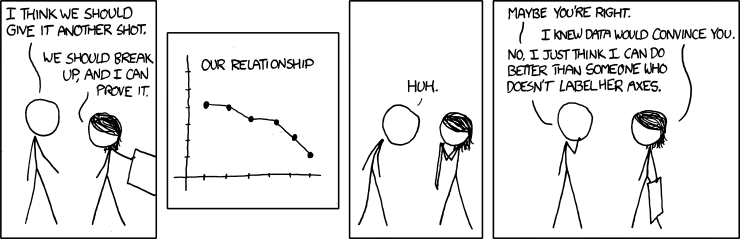
\includegraphics[scale=0.5]{images/convincing.png}
\caption{Bild von www.xkcd.com}
\end{figure}
\FloatBarrier

\begin{Antwort}
\begin{lstlisting}[style=latex]
\begin{figure}[h]
\centering
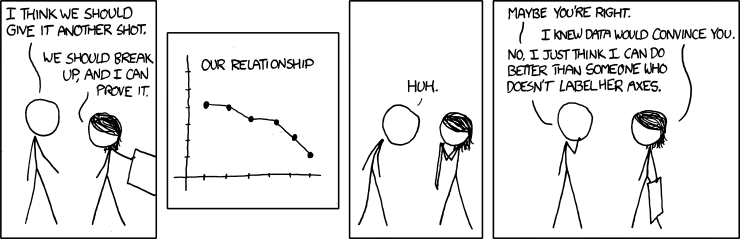
\includegraphics[scale=0.5]{images/convincing.png}
\caption{Bild von www.xkcd.com}
\end{figure}
\end{lstlisting}
\end{Antwort}

\section{Wir haben verschiedene Positionierungen für Bilder kennengelernt.}
\begin{enumerate}
\item Erstelle ein \LaTeX Dokument, dass 3 Seiten Text enthält.
\item Lade dir verschiedene Bilder runter und binde sie an verschiedenen Stellen im Text ein. Verwende dabei verschiedene Positionsangaben, die du aus der Vorlesung kennengelernt hast. Achte darauf, dass du alle Bilder beschriftest. 
%\item Recherchiere (Google) wie du ein Abbildungsverzeichnis erstellst.
\end{enumerate}



\section{Du findest auf \texttt{https://de.wikipedia.org/wiki/Diagramm} verschiedene Abbildungen von Diagrammen.}
\begin{enumerate}
\item Füge in dem Dokument aus der letzter Aufgabe, 3 dieser Abbildungen nebeneinander mit \bcode{minipages} ein.
\item Erstelle Untertitel für die Bilder. Wie kannst du die Titel über der Grafik erscheinen lassen?
\item Beobachte was sich im Abbildungsverzeichnis vergeändert hat. 
\end{enumerate}





\end{document}